\documentclass[10pt,letterpaper]{article}
\usepackage[utf8]{inputenc}
\usepackage[intlimits]{amsmath}
\usepackage{amsfonts}
\usepackage{amssymb}
\usepackage{ragged2e}
\usepackage[letterpaper, margin=0.5in]{geometry}
\usepackage{graphicx}
\usepackage{cancel}
\usepackage{mathtools}
\usepackage{tabularx}
\usepackage{arydshln}
\usepackage{tensor}
\usepackage{array}
\usepackage{xcolor}
\usepackage[boxed]{algorithm}
\usepackage[noend]{algpseudocode}
\usepackage{listings}
\usepackage{textcomp}
% \usepackage[pdf,tmpdir,singlefile]{graphviz}
\usepackage{mathrsfs}
\usepackage{bbm}
\usepackage{tikz}
\usepackage{tikz-cd}
\usepackage{enumitem}
\usepackage{arydshln}
\usepackage{relsize}
\usepackage{multirow,multicol}
\usepackage{scalerel}
\usepackage{upgreek}
\usepackage{ifthen}

\usetikzlibrary{bayesnet}
\usetikzlibrary{patterns}
\usetikzlibrary{calc}
\setlist{noitemsep}

%%%%%%%%%%%%%%%%%%%%%%%%%%%%%
% Formatting commands
%%%%%%%%%%%%%%%%%%%%%%%%%%%%%
\newcommand{\n}{\hfill\break}
\newcommand{\nn}{\vspace{0.5\baselineskip}\n}
\newcommand{\up}{\vspace{-\baselineskip}}
\newcommand{\hangblock}[2]{\par\noindent\settowidth{\hangindent}{\textbf{#1: }}\textbf{#1: }\nolinebreak#2}
\newcommand{\lemma}[1]{\hangblock{Lemma}{#1}}
\newcommand{\defn}[1]{\hangblock{Defn}{#1}}
\newcommand{\thm}[1]{\hangblock{Thm}{#1}}
\newcommand{\cor}[1]{\hangblock{Cor}{#1}}
\newcommand{\prop}[1]{\hangblock{Prop}{#1}}
\newcommand{\ex}[1]{\hangblock{Ex}{#1}}
\newcommand{\exer}[1]{\hangblock{Exer}{#1}}
\newcommand{\fact}[1]{\hangblock{Fact}{#1}}
\newcommand{\remark}[1]{\hangblock{Remark}{#1}}
\newcommand{\proven}{\;$\square$\n}
\newcommand{\problem}[1]{\par\noindent{\nolinebreak#1}\n}
\newcommand{\problempart}[2]{\par\noindent\indent{}\settowidth{\hangindent}{\textbf{(#1)} \indent{}}\textbf{(#1) }\nolinebreak#2\n}
\newcommand{\ptxt}[1]{\textrm{\textnormal{#1}}}
\newcommand{\inlineeq}[1]{\centerline{$\displaystyle #1$}}
\newcommand{\pageline}{\up\par\noindent\rule{\textwidth}{0.1pt}}

%%%%%%%%%%%%%%%%%%%%%%%%%%%%%
% Math commands
%%%%%%%%%%%%%%%%%%%%%%%%%%%%%
% Set Theory
\newcommand{\card}[1]{\left|#1\right|}
\newcommand{\set}[1]{\left\{#1\right\}}
\newcommand{\setmid}{\;\middle|\;}
\newcommand{\ps}[1]{\mathcal{P}\left(#1\right)}
\newcommand{\pfinite}[1]{\mathcal{P}^{\ptxt{finite}}\left(#1\right)}
\newcommand{\naturals}{\mathbb{N}}
\newcommand{\N}{\naturals}
\newcommand{\integers}{\mathbb{Z}}
\newcommand{\Z}{\integers}
\newcommand{\rationals}{\mathbb{Q}}
\newcommand{\Q}{\rationals}
\newcommand{\reals}{\mathbb{R}}
\newcommand{\R}{\reals}
\newcommand{\complex}{\mathbb{C}}
\newcommand{\C}{\complex}
\newcommand{\halfPlane}{\mathbb{H}}
\let\HSym\H
\let\H\relax
\newcommand{\H}{\halfPlane}
\newcommand{\comp}{^{\complement}}
\DeclareMathOperator{\Hom}{Hom}
\newcommand{\Ind}{\mathbbm{1}}
\newcommand{\cut}{\setminus}
\DeclareMathOperator{\elem}{elem}

% Differentiable Manifolds
\newcommand{\RP}{\mathbb{RP}}
\newcommand{\CP}{\mathbb{RP}}
\newcommand{\osubset}{\overset{\mathclap{\scalebox{0.5}{\ptxt{open}}}}{\subset}}
\newcommand{\osubseteq}{\overset{\mathclap{\scalebox{0.5}{\ptxt{open}}}}{\subseteq}}
\newcommand{\osupset}{\overset{\mathclap{\scalebox{0.5}{\ptxt{open}}}}{\supset}}
\newcommand{\osupseteq}{\overset{\mathclap{\scalebox{0.5}{\ptxt{open}}}}{\supseteq}}
\newcommand{\pdat}[3]{\left.\pd{#1}{#2}\right|_{#3}}
\DeclareMathOperator{\so}{so}
\DeclareMathOperator{\codim}{codim}
\DeclareMathOperator{\Diff}{Diff}
\let\dSym\d
\let\d\relax
\newcommand{\d}{\partial}
\DeclareMathOperator{\gl}{gl}
\DeclareMathOperator{\Ad}{Ad}
\newcommand{\comm}[1]{\left[#1\right]}
\DeclareMathOperator{\Fix}{Fix}

% Graph Theory
\let\deg\relax
\DeclareMathOperator{\deg}{deg}
\newcommand{\degp}{\ptxt{deg}^{+}}
\newcommand{\degn}{\ptxt{deg}^{-}}
\newcommand{\precdot}{\mathrel{\ooalign{$\prec$\cr\hidewidth\hbox{$\cdot\mkern0.5mu$}\cr}}}
\newcommand{\succdot}{\mathrel{\ooalign{$\cdot\mkern0.5mu$\cr\hidewidth\hbox{$\succ$}\cr\phantom{$\succ$}}}}
\DeclareMathOperator{\cl}{cl}
\DeclareMathOperator{\affdim}{affdim}

% Probability
\newcommand{\parSymbol}{\P}
\newcommand{\Prob}{\mathbb{P}}
\renewcommand{\P}{\Prob}
\newcommand{\Avg}{\mathbb{E}}
\newcommand{\E}{\Avg}
\DeclareMathOperator{\Var}{Var}
\DeclareMathOperator{\Cov}{Cov}
\DeclareMathOperator{\cov}{cov}
\DeclareMathOperator{\Corr}{Corr}
\DeclareMathOperator{\Unif}{Unif}
\DeclareMathOperator{\Binom}{Binom}
\newcommand{\CI}{\mathrel{\text{\scalebox{1.07}{$\perp\mkern-10mu\perp$}}}}
\DeclareMathOperator{\Ber}{Ber}
\DeclareMathOperator{\Bin}{Bin}
\DeclareMathOperator{\Geom}{Geom}
\DeclareMathOperator{\Poisson}{Poisson}
\DeclareMathOperator{\Exp}{Exp}
\DeclareMathOperator{\Beta}{Beta}
\DeclareMathOperator{\Normal}{N}
\DeclareMathOperator{\DistGamma}{Gamma}

% Standard Math
\newcommand{\inv}{^{-1}}
\newcommand{\abs}[1]{\left|#1\right|}
\newcommand{\ceil}[1]{\left\lceil{}#1\right\rceil{}}
\newcommand{\floor}[1]{\left\lfloor{}#1\right\rfloor{}}
\newcommand{\conj}[1]{\overline{#1}}
\newcommand{\of}{\circ}
\newcommand{\tri}{\triangle}
\newcommand{\inj}{\hookrightarrow}
\newcommand{\surj}{\twoheadrightarrow}
\newcommand{\ndiv}{\nmid}
\renewcommand{\epsilon}{\varepsilon}
\newcommand{\divides}{\mid}
\newcommand{\ndivides}{\nmid}
\DeclareMathOperator{\lcm}{lcm}
\DeclareMathOperator{\sgn}{sgn}
\newcommand{\map}[4]{\!\!\!\begin{array}[t]{rcl}#1 & \!\!\!\!\to & \!\!\!\!#2\\ {}#3 & \!\!\!\!\mapsto & \!\!\!\!#4\end{array}}
\newcommand{\bigsum}[2]{\smashoperator[lr]{\sum_{\scalebox{#1}{$#2$}}}}
\DeclareMathOperator{\gcf}{gcf}
\newcommand{\restr}[1]{\left.#1\right|}

% Linear Algebra
\newcommand{\Id}{\textrm{\textnormal{Id}}}
\newcommand{\im}{\textrm{\textnormal{im}}}
\newcommand{\norm}[1]{\abs{\abs{#1}}}
\newcommand{\tpose}{^{T}\!}
\newcommand{\iprod}[1]{\left<#1\right>}
\newcommand{\giprod}{\iprod{\;\,,\;}}
\DeclareMathOperator{\tr}{tr}
\DeclareMathOperator{\trace}{tr}
\newcommand{\chgBasMat}[3]{\!\!\tensor*[_{#1}]{\left[#2\right]}{_{#3}}}
\newcommand{\vecBas}[2]{\tensor*[]{\left[#1\right]}{_{#2}}}
\DeclareMathOperator{\GL}{GL}
\DeclareMathOperator{\Mat}{Mat}
\DeclareMathOperator{\vspan}{span}
\DeclareMathOperator{\rank}{rank}
\newcommand{\V}[1]{\vec{#1}}
\DeclareMathOperator{\proj}{proj}
\DeclareMathOperator{\compProj}{comp}
\DeclareMathOperator{\row}{row}
\newcommand{\smallPMatrix}[1]{\paren{\begin{smallmatrix}#1\end{smallmatrix}}}
\newcommand{\smallBMatrix}[1]{\brack{\begin{smallmatrix}#1\end{smallmatrix}}}
\newcommand{\pmat}[1]{\begin{pmatrix}#1\end{pmatrix}}
\newcommand{\bmat}[1]{\begin{bmatrix}#1\end{bmatrix}}
\newcommand{\dual}{^{*}}
\newcommand{\pinv}{^{\dagger}}
\newcommand{\horizontalMatrixLine}{\ptxt{\rotatebox[origin=c]{-90}{$|$}}}
\DeclareMathOperator{\range}{range}
\DeclareMathOperator{\Symm}{Symm}
\DeclareMathOperator{\SU}{SU}
\DeclareMathOperator{\U}{U}

% Multilinear Algebra
\let\Lsym\L
\let\L\relax
\DeclareMathOperator{\L}{\mathscr{L}}
\DeclareMathOperator{\A}{\mathcal{A}}
\DeclareMathOperator{\Alt}{Alt}
\DeclareMathOperator{\Sym}{Sym}
\newcommand{\ot}{\otimes}
\newcommand{\ox}{\otimes}
\DeclareMathOperator{\asc}{asc}
\DeclareMathOperator{\asSet}{set}
\DeclareMathOperator{\sort}{sort}
\DeclareMathOperator{\ringA}{\mathring{A}}
\DeclareMathOperator{\Sh}{Sh}
\DeclareMathOperator{\Bil}{Bil}

% Topology
\newcommand{\closure}[1]{\overline{#1}}
\newcommand{\uball}{\mathcal{U}}
\DeclareMathOperator{\Int}{Int}
\DeclareMathOperator{\Ext}{Ext}
\DeclareMathOperator{\Bd}{Bd}
\DeclareMathOperator{\rInt}{rInt}
\DeclareMathOperator{\ch}{ch}
\DeclareMathOperator{\ah}{ah}
\newcommand{\LargerTau}{\mathlarger{\mathlarger{\mathlarger{\mathlarger{\tau}}}}}
\newcommand{\Tau}{\mathcal{T}}

% Analysis
\DeclareMathOperator{\Graph}{Graph}
\DeclareMathOperator{\epi}{epi}
\DeclareMathOperator{\hypo}{hypo}
\DeclareMathOperator{\supp}{supp}
\newcommand{\lint}[2]{\underset{#1}{\overset{#2}{{\color{black}\underline{{\color{white}\overline{{\color{black}\int}}\color{black}}}}}}}
\newcommand{\uint}[2]{\underset{#1}{\overset{#2}{{\color{white}\underline{{\color{black}\overline{{\color{black}\int}}\color{black}}}}}}}
\newcommand{\alignint}[2]{\underset{#1}{\overset{#2}{{\color{white}\underline{{\color{white}\overline{{\color{black}\int}}\color{black}}}}}}}
\newcommand{\extint}{\ptxt{ext}\int}
\newcommand{\extalignint}[2]{\ptxt{ext}\alignint{#1}{#2}}
\newcommand{\conv}{\ast}
\newcommand{\pd}[2]{\frac{\partial{}#1}{\partial{}#2}}
\newcommand{\del}{\nabla}
\DeclareMathOperator{\grad}{grad}
\DeclareMathOperator{\curl}{curl}
\let\div\relax
\DeclareMathOperator{\div}{div}
\DeclareMathOperator{\vol}{vol}

% Complex Analysis
\let\Re\relax
\DeclareMathOperator{\Re}{Re}
\let\Im\relax
\DeclareMathOperator{\Im}{Im}
\DeclareMathOperator{\Res}{Res}

% Abstract Algebra
\DeclareMathOperator{\ord}{ord}
\newcommand{\generated}[1]{\left<#1\right>}
\newcommand{\cycle}[1]{\smallPMatrix{#1}}
\newcommand{\id}{\ptxt{id}}
\newcommand{\iso}{\cong}
\DeclareMathOperator{\Aut}{Aut}
\DeclareMathOperator{\SL}{SL}
\DeclareMathOperator{\op}{op}
\newcommand{\isom}[4]{\!\!\!\begin{array}[t]{rcl}#1 & \!\!\!\!\overset{\sim}{\to} & \!\!\!\!#2\\ #3 & \!\!\!\!\mapsto & \!\!\!\!#4\end{array}}
\newcommand{\F}{\mathbb{F}}
\newcommand{\acts}{\;\reflectbox{\rotatebox[origin=c]{-90}{$\circlearrowright$}}\;}
\newcommand{\disjunion}{\mathrel{\text{\scalebox{1.07}{$\perp\mkern-10mu\perp$}}}}
\DeclareMathOperator{\SO}{SO}
\DeclareMathOperator{\stab}{stab}
\DeclareMathOperator{\nullity}{nullity}
\DeclareMathOperator{\Perm}{Perm}
\DeclareMathOperator{\nsubgp}{\vartriangleleft}
\DeclareMathOperator{\notnsubgp}{\ntriangleleft}
\newcommand{\presentation}[2]{\left<#1\;\middle|\;#2\right>}
\DeclareMathOperator{\Char}{char}
\DeclareMathOperator{\fchar}{char}
\DeclareMathOperator{\triv}{triv}
\DeclareMathOperator{\reg}{reg}
\DeclareMathOperator{\std}{std}
\DeclareMathOperator{\Func}{Func}
\DeclareMathOperator{\End}{End}

% Convex Optimization
\let\sectionSymbol\S
\let\S\relax
\newcommand{\S}{\mathbb{S}}
\DeclareMathOperator{\dist}{dist}
\DeclareMathOperator{\dom}{dom}
\DeclareMathOperator{\diag}{diag}
\DeclareMathOperator{\ones}{\mathbbm{1}}
\newcommand{\minimizeOver}[3]{\begin{array}{rl}\underset{#1}{\ptxt{minimize}} & #2\\ \ptxt{subject to} & #3\end{array}}
\newcommand{\maximizeOver}[3]{\begin{array}{rl}\underset{#1}{\ptxt{maximize}} & #2\\ \ptxt{subject to} & #3\end{array}}
\newcommand{\minimizationProblem}[2]{\minimizeOver{}{#1}{#2}}
\newcommand{\maximizationProblem}[2]{\maximizeOver{}{#1}{#2}}
\newcommand{\minimizeOverUnconstrained}[2]{\begin{array}{rl}\underset{#1}{\ptxt{minimize}} & #2\end{array}}
\newcommand{\maximizeOverUnconstrained}[2]{\begin{array}{rl}\underset{#1}{\ptxt{maximize}} & #2\end{array}}
\newcommand{\minimizationUnconstrained}[1]{\minimizeOverUnconstrained{}{#1}}
\newcommand{\maximizationUnconstrained}[1]{\maximizeOverUnconstrained{}{#1}}
\DeclareMathOperator{\argmin}{argmin}
\DeclareMathOperator{\argmax}{argmax}

% Proofs
\newcommand{\st}{s.t.}
\newcommand{\unique}{!}
\newcommand{\iffdef}{\overset{\ptxt{def}}{\Leftrightarrow}}
\newcommand{\eqVertical}{\rotatebox[origin=c]{90}{=}}
\newcommand{\mapsfrom}{\mathrel{\reflectbox{\ensuremath{\mapsto}}}}
\newcommand{\mapsdown}{\rotatebox[origin=c]{-90}{$\mapsto$}\mkern2mu}
\newcommand{\mapsup}{\rotatebox[origin=c]{90}{$\mapsto$}\mkern2mu}
\newcommand{\from}{\!\mathrel{\reflectbox{\ensuremath{\to}}}}
\newcommand{\labeledeq}[1]{\overset{\mathclap{\ptxt{#1}}}{=}}
\newcommand{\eqdef}{\labeledeq{def}}

% Brackets
\newcommand{\paren}[1]{\left(#1\right)}
\renewcommand{\brack}[1]{\left[#1\right]}
\renewcommand{\brace}[1]{\left\{#1\right\}}
\newcommand{\ang}[1]{\left<#1\right>}

% Algorithms
\algrenewcommand{\algorithmiccomment}[1]{\hskip 1em \texttt{// #1}}
\algrenewcommand\algorithmicrequire{\textbf{Input:}}
\algrenewcommand\algorithmicensure{\textbf{Output:}}
\newcommand{\algP}{\ptxt{\textbf{P}}}
\newcommand{\algNP}{\ptxt{\textbf{NP}}}
\newcommand{\algNPC}{\ptxt{\textbf{NP-Complete}}}
\newcommand{\algNPH}{\ptxt{\textbf{NP-Hard}}}
\newcommand{\algEXP}{\ptxt{\textbf{EXP}}}
\DeclareMathOperator{\fl}{fl}

%%%%%%%%%%%%%%%%%%%%%%%%%%%%%
% Other commands and shorthand
%%%%%%%%%%%%%%%%%%%%%%%%%%%%%
\newcommand{\flag}[1]{\textbf{\textcolor{red}{#1}}}
\let\uSym\u
\let\u\relax
\newcommand{\u}[1]{\underline{#1}}
\let\bSym\b
\let\b\relax
\newcommand{\b}[1]{\textbf{#1}}
\let\iSym\i
\let\i\relax
\newcommand{\i}[1]{\textit{#1}}
\let\scSym\sc
\let\sc\relax
\newcommand{\sc}[1]{\textsc{#1}}
\newcommand{\mf}[1]{\mathfrak{#1}}
\newcommand{\mc}[1]{\mathcal{#1}}

%%%%%%%%%%%%%%%%%%%%%%%%%%%%%%%%%%%%%%%
% Make l's curvy in math environments %
%%%%%%%%%%%%%%%%%%%%%%%%%%%%%%%%%%%%%%%
\mathcode`l="8000
\begingroup
\makeatletter
\lccode`\~=`\l
\DeclareMathSymbol{\lsb@l}{\mathalpha}{letters}{`l}
\lowercase{\gdef~{\ifnum\the\mathgroup=\m@ne \ell \else \lsb@l \fi}}%
\endgroup

%%%%%%%%%%%%%%%%%%%%%%%%%
% Fix \vdots and \ddots %
%%%%%%%%%%%%%%%%%%%%%%%%%
\usepackage{letltxmacro}
\LetLtxMacro\orgvdots\vdots
\LetLtxMacro\orgddots\ddots

\makeatletter
\DeclareRobustCommand\vdots{%
	\mathpalette\@vdots{}%
}
\newcommand*{\@vdots}[2]{%
	% #1: math style
	% #2: unused
	\sbox0{$#1\cdotp\cdotp\cdotp\m@th$}%
	\sbox2{$#1.\m@th$}%
	\vbox{%
		\dimen@=\wd0 %
		\advance\dimen@ -3\ht2 %
		\kern.5\dimen@
		% remove side bearings
		\dimen@=\wd2 %
		\advance\dimen@ -\ht2 %
		\dimen2=\wd0 %
		\advance\dimen2 -\dimen@
		\vbox to \dimen2{%
			\offinterlineskip
			\copy2 \vfill\copy2 \vfill\copy2 %
		}%
	}%
}
\DeclareRobustCommand\ddots{%
	\mathinner{%
		\mathpalette\@ddots{}%
		\mkern\thinmuskip
	}%
}
\newcommand*{\@ddots}[2]{%
	% #1: math style
	% #2: unused
	\sbox0{$#1\cdotp\cdotp\cdotp\m@th$}%
	\sbox2{$#1.\m@th$}%
	\vbox{%
		\dimen@=\wd0 %
		\advance\dimen@ -3\ht2 %
		\kern.5\dimen@
		% remove side bearings
		\dimen@=\wd2 %
		\advance\dimen@ -\ht2 %
		\dimen2=\wd0 %
		\advance\dimen2 -\dimen@
		\vbox to \dimen2{%
			\offinterlineskip
			\hbox{$#1\mathpunct{.}\m@th$}%
			\vfill
			\hbox{$#1\mathpunct{\kern\wd2}\mathpunct{.}\m@th$}%
			\vfill
			\hbox{$#1\mathpunct{\kern\wd2}\mathpunct{\kern\wd2}\mathpunct{.}\m@th$}%
		}%
	}%
}
\makeatother

\newcommand{\B}{
	
\begin{tikzpicture}
	\filldraw [fill=red, draw=black] (0, 0) rectangle (0.37, 0.45);
	\draw [line width=0.5mm, white ] (0.1,0.08) -- (0.1,0.38);
	\draw[line width=0.5mm, white ] (0.1, 0.35) .. controls (0.2, 0.35) and (0.4, 0.2625) .. (0.1, 0.225);
	\draw[line width=0.5mm, white ] (0.1, 0.225) .. controls (0.2, 0.225) and (0.4, 0.1625) .. (0.1, 0.1);
	\end{tikzpicture}
}

% Allow custom symbols as arrows in tikz-cd
\tikzset{
  symbol/.style={
    draw=none,
    every to/.append style={
      edge node={node [sloped, allow upside down, auto=false]{$#1$}}}
  }
}
% Example: \arrow[r,symbol=\cong]
% https://tex.stackexchange.com/questions/394154/how-to-include-inclusion-subgroup-relationship-in-tikz-cd-diagram

\author{Thomas Cohn}
\title{Math 635 Lecture 17}
\date{3/1/21} % Can also use \today

\begin{document}
\maketitle
\setlength\RaggedRightParindent{\parindent}
\RaggedRight

\par\noindent
Recall the setup from last time:

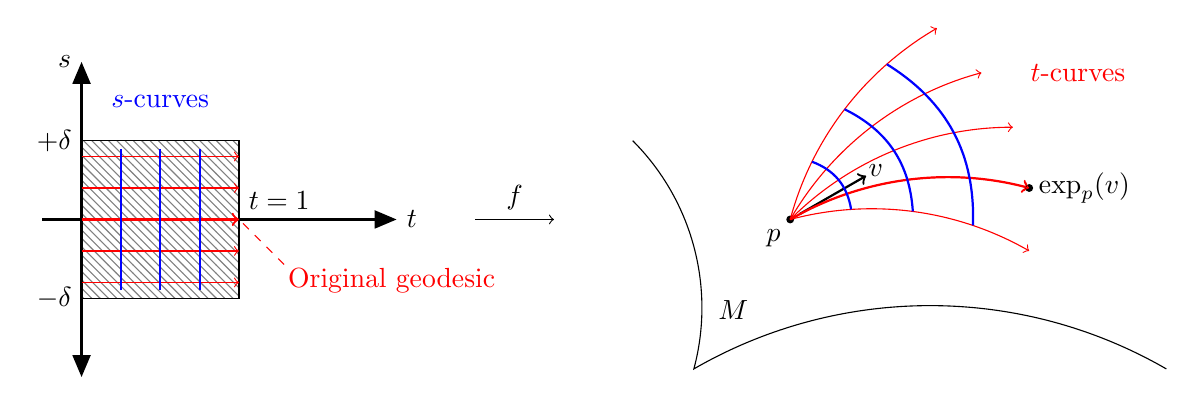
\begin{tikzpicture}
	\draw[pattern=north west lines, pattern color=gray] (0,-1) rectangle (2,1);
	\draw[thick, ->] (-0.5,0) -- (4,0) node[anchor=west]{$t$};
	\draw[thick, <->] (0,-2) -- (0,2) node[anchor=east]{$s$};
	\draw (0,1) node[anchor=east]{$+\delta$} -- (2,1) -- (2,-1) -- (0,-1) node[anchor=east]{$-\delta$};
	\draw[-to, thick, red] (0,0) -- (2,0);
	\draw[-to, red] (0,0.4) -- (2,0.4);
	\draw[-to, red] (0,0.8) -- (2,0.8);
	\draw[-to, red] (0,-0.4) -- (2,-0.4);
	\draw[-to, red] (0,-0.8) -- (2,-0.8);
	\draw[thick, blue] (0.5,-0.9) -- (0.5,0.9);
	\draw[thick, blue] (1,-0.9) -- (1,0.9);
	\draw[thick, blue] (1.5,-0.9) -- (1.5,0.9);
	%
	\draw[-to] (5,0) -- (6,0);
	%
	\draw (7,1) arc (45:-15:3) node (M) {} arc (120:60:6);
	\node (p) at (9,0) {};
	\fill (p) circle [radius=0.05cm];
	\draw (p) + ({1.25*0.87}, {1.25*0.5}) node (v) {};
	\draw[-to, thick] (p) -- (v);
	\draw[-to, red] (p) arc (105:93.75:4) node (s11) {} arc (93.75:82.5:4) node (s21) {} arc (82.5:71.25:4) node (s31) {} arc (71.25:60:4);
	\draw[-to, red, thick] (p) arc (120:75:4) node (exppv) {};
	\draw[-to, red] (p) arc (135:90:4);
	\draw[-to, red] (p) arc (150:105:4) node (tcurve) {};
	\draw[-to, red] (p) arc (165:153.75:4) node (s12) {} arc (153.75:142.5:4) node (s22) {} arc (142.5:131.25:4) node (s32) {} arc (131.25:120:4);
	\fill (exppv) circle [radius=0.05cm];
	\draw[-to, red] (p) arc (120:75:4);
	\draw[blue, thick, bend right=30] (s11.center) to (s12.center);
	\draw[blue, thick, bend right=30] (s21.center) to (s22.center);
	\draw[blue, thick, bend right=30] (s31.center) to (s32.center);
	%
	\draw (5.5,0) node[anchor=south]{$f$};
	\draw (p) node[anchor=north east]{$p$};
	\draw (v) + (0,0) node {$v$};
	\draw (exppv) node[anchor=west]{$\exp_{p}(v)$};
	\draw[red] (tcurve) + (0.5,0) node[anchor=west]{$t$-curves};
	\draw[red] (2.5,-0.5) node[anchor=north west] {Original geodesic};
	\draw[red, dashed] (2.05,-0.05) -- (2.6,-0.6);
	\draw[blue] (1,1.5) node {$s$-curves};
	\draw (2,0) node[anchor=south west]{$t=1$};
	\draw (M) + (0.5,0.75) node{$M$};
\end{tikzpicture}

\defn{
	A \u{vector field along $f$} is a lift $\tilde{f}$ of $f$ to $TM$. I.e., $\tilde{f}$ is defined such that the following diagram commutes:
	\[
		\begin{tikzcd}[ampersand replacement=\&]
			\& TM\arrow[d,"\pi"] \\[-10pt]
			D \arrow[ur,"\tilde{f}"] \arrow[r,"f"'] \& M
		\end{tikzcd}
	\]
}

\par\noindent
Note that such a lift isn't unique!\n

\ex{
	One such lift is $\displaystyle\tilde{f}=\left\{\begin{array}{l}f_{t}\\ f_{s}\end{array}\right.$. For such a $\tilde{f}$, we can define $\frac{D}{dt}\tilde{f}$ and $\frac{D}{ds}\tilde{f}$ by restricting $\tilde{f}$ to $t$ and $s$ curves, respectively.\n
}

\prop{
	$\frac{D}{dt}f_{s}=\frac{D}{ds}f_{t}$ at each $(t,s)$.\nn
	Proof: We will compute in local coordinates $(x^{1},\ldots,x^{n})$. Let $X_{i}=\pd{}{x^{i}}$, $\forall{}i$. We write $f(t,s)=(x^{1}(t,s),\ldots,x^{n}(t,s))$, where $x^{i}(t,s):\dom(f)\to\R$. Note that we can write $f_{s}=\pd{x^{i}}{s}X_{i}(f(t,s))$, and likewise for $f_{t}$. We now compute
	\[
		\frac{D}{dt}f_{s}=\frac{\d^{2}x^{i}}{\d{}t\d{}s}X_{i}+\pd{x^{i}}{s}\frac{D}{dt}X_{i}
	\]
	We know $f_{t}=\pd{x^{j}}{t}X_{j}$, so because $\frac{D}{dt}$ is the covariant derivative with respect to $f_{t}$,
	\[
		\frac{D}{dt}X_{i}=\pd{x^{j}}{t}\nabla_{X_{j}}X_{i}\qquad\frac{D}{dt}f_{s}=\frac{\d^{2}x^{i}}{\d{}t\d{}s}X_{i}+\pd{x^{i}}{s}\pd{x^{j}}{t}\nabla_{X_{j}}X_{i}
	\]
	Computing similarly, we also get
	\[
		\frac{D}{ds}f_{t}=\frac{\d^{2}x^{i}}{\d{}s\d{}t}X_{i}+\pd{x^{i}}{t}\pd{x^{j}}{s}\nabla_{X_{j}}X_{i}
	\]
	By Clairaut's theorem, $\frac{\d^{2}x^{i}}{\d{}t\d{}s}=\frac{\d^{2}x^{i}}{\d{}s\d{}t}$, so the first term of $\frac{D}{dt}f_{s}$ and $\frac{D}{ds}f_{t}$ are equal. Furthermore, because the Levi-Civita connection is torsion-free, $\comm{X_{i},X_{j}}=0$, so $\nabla_{X_{j}}X_{i}=\nabla_{X_{i}}X_{j}$. This means we can swap the coefficients in the second term to show equality. We conclude that $\frac{D}{dt}f_{s}=\frac{D}{ds}f_{t}$.\proven
}

\par\noindent
Observe: We can ask if $\frac{D}{ds}$ and $\frac{D}{dt}$ commute. We'll see on Friday that the answer is no, because curvature comes into play.\n

\par\noindent
We're now ready to prove Gauss' lemma...\newpage

\lemma{
	(Gauss' Lemma) In a normal neighborhood of $p$, radial geodesics are orthogonal to geodesic spheres.\nn
	Proof: Let $p\in{}M$ and $\varepsilon>0$ such that $\exp_{p}:B_{\varepsilon}(0)\overset{\sim}{\to}\exp_{p}(B_{\varepsilon}(0))$ (with $B_{\varepsilon}(0)\subseteq{}T_{p}M$ and $\exp_{p}(B_{\varepsilon}(0))\subseteq{}M$) is a diffeomorphism onto its image. Take $r\in(0,\varepsilon)$, so $S_{r}\subseteq{}T_{p}M$ is the sphere of radius $r$. Then choose any curve $s\mapsto{}c(s)\in{}S_{r}$, for an arbtirarily small domain $s\in(-\delta,\delta)$. Define $f(t,s)=\exp_{p}(tc(s))$. Illustration:\n
	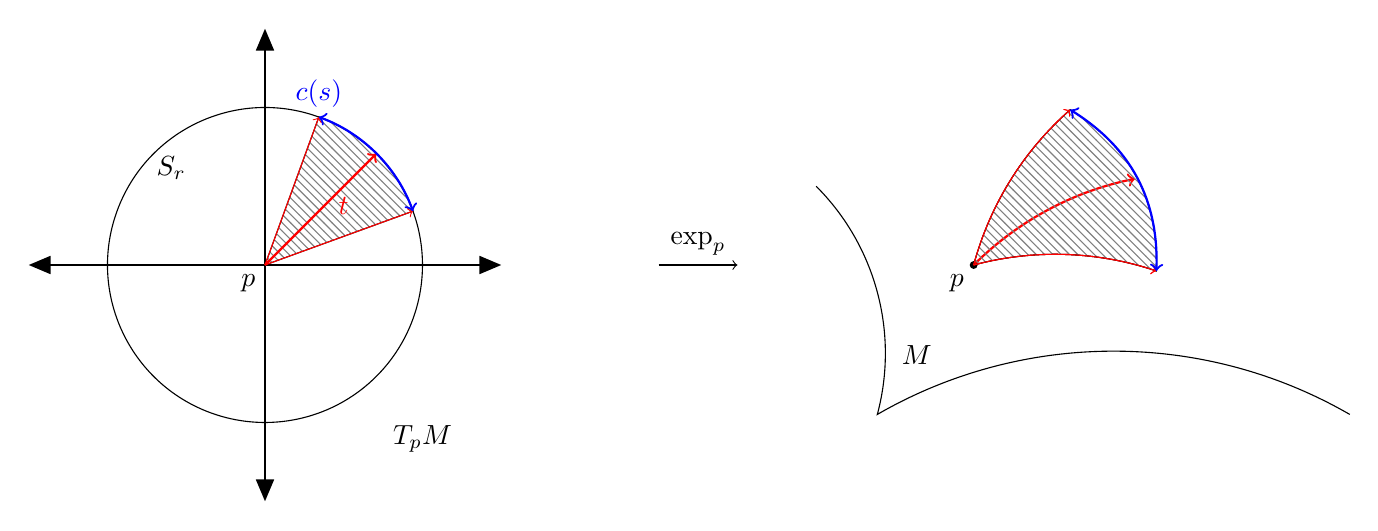
\begin{tikzpicture}
		\draw[thick, <->] (-3,0) -- (3,0);
		\draw[thick, <->] (0,-3) -- (0,3);
		\draw (2,0) arc (0:20:2) node (c1) {} arc (20:45:2) node (c2) {} arc (45:70:2) node (c3) {} arc (70:360:2);
		\draw[pattern=north west lines, pattern color=gray] (0,0) -- (c1.center) arc (20:70:2) -- cycle;
		\draw[red, -to] (0,0) -- (c1.center);
		\draw[red, thick, -to] (0,0) -- (c2.center);
		\draw[red, -to] (0,0) -- (c3.center);
		\draw[to-to, thick, blue] (c1.center) arc (20:70:2);
		%
		\draw[-to] (5,0) -- (6,0);
		%
		\draw (7,1) arc (45:-15:3) node (M) {} arc (120:60:6);
		\node (p) at (9,0) {};
		\fill (p) circle [radius=0.05cm];
		\draw[-to, red] (p) arc (105:93.75:4) node (s11) {} arc (93.75:82.5:4) node (s21) {} arc (82.5:71.25:4) node (s31) {};
		\draw[-to, red, thick] (p) arc (135:101.25:4);
		\draw[-to, red] (p) arc (165:153.75:4) node (s12) {} arc (153.75:142.5:4) node (s22) {} arc (142.5:131.25:4) node (s32) {};
		\draw[pattern=north west lines, pattern color=gray] (p.center) arc (105:71.25:4) to[bend right=30] (s32.center) arc (131.25:165:4);
		\draw[-to, red] (p) arc (105:93.75:4) arc (93.75:82.5:4) arc (82.5:71.25:4);
		\draw[-to, red] (p) arc (165:153.75:4) arc (153.75:142.5:4) arc (142.5:131.25:4);
		\draw[blue, thick, bend right=30, to-to] (s31.center) to (s32.center);
		%
		\draw (5.5,0) node[anchor=south]{$\exp_{p}$};
		\draw (p) node[anchor=north east]{$p$};
		\draw (M) + (0.5,0.75) node{$M$};
		\draw (2.5,-2.5) node[anchor=south east] {$T_{p}M$};
		\draw[blue] (c3) node[anchor=south] {$c(s)$};
		\draw[red] (1,0.75) node {$t$};
		\draw (-1.5,1.5) node[anchor=north west] {$S_{r}$};
		\draw (0,0) node[anchor=north east] {$p$};
	\end{tikzpicture}\n
	The key calculation we'll perform is $\frac{d}{dt}\iprod{f_{t},f_{s}}$; we want to show it's equal to $0$. Well,
	\begin{align*}
		\frac{d}{dt}\iprod{f_{t},f_{s}} & =\iprod{\frac{D}{dt}f_{t},f_{s}}+\iprod{f_{t},\frac{D}{dt}f_{s}}\\
		& \labeledeq{(1)}\iprod{0,f_{s}}+\iprod{f_{t},\frac{D}{dt}f_{s}}\\
		& =\iprod{f_{t},\frac{D}{dt}f_{s}}\\
		& \labeledeq{(2)}\iprod{f_{t},\frac{D}{ds}f_{t}}\\
		& =\frac{1}{2}\iprod{\frac{D}{ds}f_{t},f_{t}}+\frac{1}{2}\iprod{f_{t},\frac{D}{ds}f_{t}}\\
		& =\frac{1}{2}\frac{d}{ds}\iprod{f_{t},f_{t}}\\
		& \labeledeq{(3)}\frac{1}{2}\frac{d}{ds}\norm{c(s)^{2}}\\
		& =\frac{1}{2}\frac{d}{ds}r^{2}\\
		& =0
	\end{align*}
	with (1) because $t\mapsto\exp_{p}(tv)=G(1,p,tv)=G(t,p,v)$ is a geodesic, (2) because of the proposition from earlier, and (3) because $\iprod{f_{t},f_{t}}$ is constant with repsect to $t$, so we can choose to evaluate it at $t=0$. Now, we can evaluate $\restr{\iprod{f_{t},f_{s}}}_{t=0}=\iprod{c(s),0}=0$, so we get that, for all $t,s$, $\iprod{f_{t},f_{s}}=0$.\proven
}

\par\noindent
Why are we done? Well, we can find $f_{t}(t)$ by $f(t,s=0)$ WOLOG, so $f(t,0)$ is the velocity of the radial geodeisc $t\mapsto\exp_{p}(tv(0))$, and $f(t,0)$ is an arbitrary tangent vector to the geodesic sphere $\exp_{p}(S_{r})$. So we conclude that the tangent space of a point $q$ on the geodesic sphere is perpendicular to the geodesic $\exp_{p}(tv)$, where $\exp_{p}(v)=q$.\newpage

\cor{
	If $U=\exp_{p}(B_{\varepsilon}(0))$ is a normal neighborhood of $p$, and $q\in{}U$, then the shortest path from $p$ to $q$ is $t\mapsto\exp_{p}(tv)$ ($0\le{}t\le{}1$), where $\exp_{p}(v)=q$. (By path, we mean a continuous, piecewise smooth function, although we only need it to be $C^{1}$ for this proof.)\nn
	Proof: Assume $c:[0,1]\to{}U$, with $c(0)=p$ and $c(1)=q$, is a smooth path, and its image is contained in $U$. Write $(\exp_{p})\inv(c(t))=r(t)w(t)$, where $r(t)\ge{}0$ and $\norm{w(t)}\equiv{}1$. Consider the family $f(r,t)=\exp_{p}(rw(t))$, so that $c(t)=f(r(t),t)$. Then $\frac{dc}{dt}=\frac{dr}{dt}f_{r}+f_{t}$, and $f_{r}$ and $f_{t}$ are perpendicular for all $t$, so we can use the Pythagorean theorem to find
	\[
		\norm{\frac{dc}{dt}}^{2}=\norm{\frac{dr}{dt}f_{r}}^{2}+\norm{f_{t}}^{2}=\abs{\frac{dr}{dt}}^{2}\norm{f_{r}}^{2}+\norm{f_{t}}^{2}=\abs{\frac{dr}{dt}}^{2}+\norm{f_{t}}^{2}\ge\abs{\frac{dr}{dt}}^{2}
	\]
	Using this inequality, we can bound the length of $c$:
	\[
		l(c)=\int_{0}^{1}\norm{\frac{dc}{dt}}\,dt\ge\int_{0}^{1}\abs{\frac{dr}{dt}}\,dt\ge\int_{0}^{1}\frac{dr}{dt}\,dt=r(1)-r(0)=r(1)
	\]
	But $r(t)$ is the length of the radial geodesic $r\mapsto\exp_{p}(rw(1))$, joining $p$ to $q$. (Note that equality holds iff $\norm{f_{t}}^{2}\equiv{}0$, which is true iff $c$ is the radial geodesic.)\nn
	Now, we must consider the case where the image of $c$ is not contained in $U$. Well, there must be some $t_{0}\in(0,1)$ \st{} $c(t_{0})$ is on the geodesic sphere psasing through $q$. We know the length of $c:[0,t_{0}]$ is no smaller than the length of a radial geodesic directly to $q$, so the inequality still holds. See the illustration below:\n
	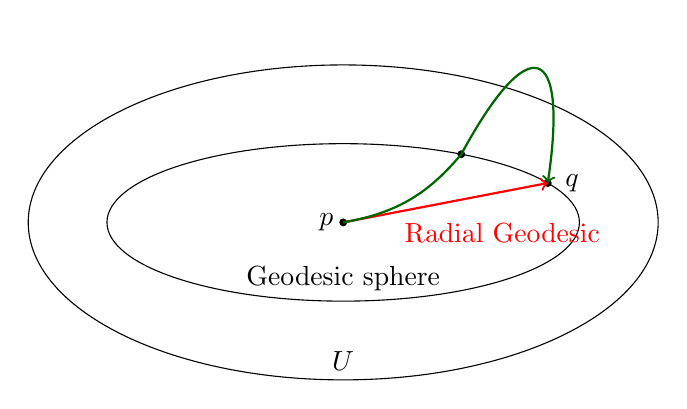
\begin{tikzpicture}
		\draw (0,0) node (p) {};
		\fill (p) circle (0.05);
		\draw (p) ellipse (3 and 1);
		\draw (p) ellipse (4 and 2);
		\node (q) at ($(0,0) + (30:3 and 1)$) {};
		\node (m) at ($(0,0) + (60:3 and 1)$) {};
		\fill (q) circle (0.05);
		\fill (m) circle (0.05);
		\draw[red, thick, -to] (0,0) -- (q.center) node[near start,anchor=north west] {Radial Geodesic};
		\draw[black!60!green, thick, -to] (0,0) to[bend right=20] (m.center) to[bend left=80, looseness=4] (q.center);
		%
		\draw (p) node[anchor=east] {$p$};
		\draw (0,-1) node[anchor=south] {Geodesic sphere};
		\draw (0,-2) node[anchor=south] {$U$};
		\draw (q) + (0.1,0) node[anchor=west] {$q$};
	\end{tikzpicture}\n
}

\cor{
	$d(p,q)=\inf(l(c))$, over the set of all $c$ joining $p$ and $q$, is actually a distance function.\n
}

\par\noindent
We showed all the other parts earlier -- the only thing left to check is that $d(p,q)=0\;\Rightarrow\;p=q$. We'll prove this by contraposition next time, but the idea is to assume that $p$ and $q$ are distinct, and then construct a normal neighborhood of $p$ that doesn't contain $q$. Then we know that $d(p,q)$ must be larger than the radius of the geodesic sphere, which is nonzero.\n

\end{document}